%Figure~\ref{figure:pipeline} depicts the summarized pipeline of the proposed method. This pipeline contains two main steps: first, the application of 1D-to-2D signal projections, where the 1D signal is transformed into a 2D image, and, then, the application of a \gls{CVC} algorithm to classify the quality of signal into reliable/not-reliable. The 1D-to-2D projection can be performed by using \gls{mtf}, \gls{rp}, or \gls{gaf} algorithms. 


%Moreover, the image aggregation of those three methods, \acrfull{PM}, was used in the scope of this work. It assigns the beforementioned projection methods images to each of the RGB channels. To the best of our knowledge, no previous work has considered a \gls{PM} yet.



%The signal projection approach can produce competitive results with state of art approaches, as using \acrshort{gaf} in combination with Vision Transformer \acrshort{ml} model \cite{1d-to-2d-freitas}. Thereby, they must be described in the following sections, starting with the latest mentioned.


%\begin{figure*}[t!]
%    \centering
%    \includegraphics[width=\linewidth]{imgs/pipeline4.png}
%    \caption{ Proposed pipeline for \acrshort{SQA} using 1D-to-2D projections in combination with \acrshort{CVC}.}
%    \label{figure:pipeline}
%\end{figure*}



% \subsection{Projection Mixture}

% Also, the aforementioned 3 projection methods were combined by image aggregation, feeding the neural networks with an image of 3 channels (usually bijective to the RGB attributes), where each channel is a projection obtained from the same signal.

%The motivation of \gls{rp} usage to project 1D signal into a \gls{2D} space by embedding procedures is to identify time recurrences (correlations) that are not easily apparent in the \gls{1D} signals. These recurrences encode physiological states that can be assessed by searching repeated patterns in the produced 2D images. Similarly, \gls{mtf} can be employed to produce such representation, but by using a Markov chain of first order. Finally, the same end can be achieved using \gls{gaf}, which represents a time series in a polar coordinate system and then it builds a Gramian matrix where each element is the trigonometric sum between different time intervals. In the Gramian matrix, each element is, actually, the cosine of the summation of angles. These algorithms are suitable for characterizing signal quality because the images generated from them produce texture patterns highly correlated with the original waveform of the 1D signal. From Figure~\ref{fig:signals_and_maps}, we can notice that a noisy signal, customarily associated with ‘unreliable’ \gls{SQI}, often presents visual patterns with lower redundancies and higher entropy. On the other hand, reliable signals usually produce projections (or `encoding maps') with lower entropy and harmonious texture patterns.

%% OBSERVATION
%% Podemos omitir para o WCOMP, mas pode detalhar ainda mais na sua dissertação!
%\subsection{Gramian Angular Field}

% The main idea behind \acrfull{gaf} projection method is utilizing the polar coordinate system $ [0,\pi] \times \mathbb{R} $, to represent the signal in a way that the overall shape of the signal curve changes as time passes, since the arc of the circumference increases as the radius increases. Therefore, not mattering if the signal is periodical, its shape changes as time passes. 

% To map a linear signal to such a coordinate system, the following identities were applied to obtain the radius $r_i$ and the angle $\phi_i$ of the $i$-th sample of the signal: ${\phi_i = arccos(x_i)}$, with ${x_i \in \mathbb{R}}, {-1 \leq x_i \leq +1}$; and ${r_i = t_i/N, t_i \in \mathbb{N}}$, with ${N \in \mathbb{R}}$, where $N$ can be used to stretch or to detract the signal along the radius axis. Notice that the signal needs to be rescaled to the interval $[-1,+1]$. 

% However, the signal is yet one-dimensional. Hence, an aggregate operation $Agg$ is applied to each pair to produce the matrix $ GAF = \{Agg(\phi_i,\phi_j)\}_{i,j}$. Examples of those aggregate functions are the $cos(\phi_i + \phi_j)$ function, which produces the Gramian Summation Angular Field ($GAF_S$), and the function $sin(\phi_i - \phi_j)$, that produces the Gramian Difference Angular Field ($GAF_D$). They can be simplified by the use of trigonometric properties, as seen in the following equations:
% \begin{align}
%     GAF_S & = (\vec{x}^T \cdot \vec{x}) - ((\Delta(\vec{x}))^T \cdot \Delta(\vec{x})) = 
%     \cos^{-1}\left( \frac{T_{ij}}{\sqrt{T_{ii} \cdot T_{jj}}} \right) \\
%     GAF_D & = ((\Delta(\vec{x}))^T \cdot \vec{x}) - (\vec{x}^T \cdot \Delta(\vec{x})) = 
%     \sin^{-1}\left( \frac{T_{ij}}{\sqrt{T_{ii} \cdot T_{jj}}} \right)
% \end{align}
% Where $\Delta(\vec{v})$ applies the function $f(x)=\sqrt{1-x^2}$ to $\vec{v}$ element-wise. 

% \subsection{Markov Transition Field}

% The Markov Transition Field's first step is elaborating a Markov chain of first order, considering as states quantile bins containing samples of the signal and defining as a transition of states $S_i \rightarrow S_j$ as the probability of, given the set of all pairs $(x_u,x_{u+1})$ of subsequent signal samples for all $x_u \in q_i$, the subsequent sample $x_{u+i}$ belong to the quantile $q_j$. Then, the Markov chain can be described as the matrix ${M = \{P(S^\prime \rightarrow S_j|S^\prime=S_i)\}_{i,j}}$, where $S^\prime$ is the current state of the Markov chain state machine. Notice that $\sum_j P(S^\prime \rightarrow S_j|S^\prime=S_i) = 1$ for each state $S_i$.

% Nonetheless, the matrix $M$ doesn't fully retain the time sequentiality, since quantiles are sets obtained by value, not by timestamp. For that reason, a second step is made, building a matrix corresponding to the Markov Transition Field, defined as follows:
% \begin{equation}
%     MTF = \{M_{u,v} | x_i \in q_u, x_j \in q_v\}_{i,j}
% \end{equation}
% Where $M_{u,v}$ is the element of the matrix M on the given row and column.

% \subsection{Recurrence Plot}

% Finally, the last method is described, beginning with the transformation of the original signal $\vec{x}_{1 \times n}$ into a matrix $X_{d \times m}$, with $m=n-(d-1)$, where each of the $m$ columns corresponds to a vector $\vec{v}_j$ of $d$ dimensions, such that $\vec{v}_j=[x_j,x_{j+\tau},...,x_{j+\tau \cdot (d-1)}]$, that is, $\vec{v}_j$ is a sequence of $d$ samples of $\vec{x}$, beginning in the position $j$, with time delays of value $\tau$ between them. From that point of view, the matrix $X_{d \times m}$ can be seen as a vector $\vec{X}_m$ with elements of $d$ dimension.

% In the end, each distance between vectors contained in $\vec{X}$ can be compared, leading to the following matrix:
% \begin{equation}
%     RP = \{ D(\vec{X}_i, \vec{X}_j)  \}_{i,j}
% \end{equation}
% Where $D(\vec{X}_i, \vec{X}_j) = || \vec{X}_i - \vec{X}_j ||$. Optionally, it's possible to apply a threshold function $\Theta$ to classify the obtained distances, resulting in the matrix $RP = \{ \Theta(D(\vec{X}_i, \vec{X}_j))  \}_{i,j}$.

This chapter first presents the overview of the method. Then, it describes the fundamental concepts about the matrix projection methods. Finally, it defines the new projection combination technique.

\section{Overview of the Proposed Method}

The Figure \ref{fig:method} depicts the application framework of this thesis. First, we transform the signal into four projections using the three before-mentioned algorithms: \gls{GAF} (which generates two variants: \gls{GASF} and \gls{GADF}, \gls{MTF}, and \gls{RP}. Then, we aggregate those projections using composition, that is, we assign each of them to a different channel of a new input layer. Then, that layer feeds the computer vision model, which contained weights pre-trained on the ImageNet dataset. The Figure \ref{fig:input_layer} pictures the feeding process to a three-channeled \gls{CV} model, which consists in performing a point-wise convolution operation. Finally, that model classifies the signal into a binary \gls{SQI}, which indicates if the signal is `Good' or `Bad'. 

\begin{figure}[t]
	\centering
	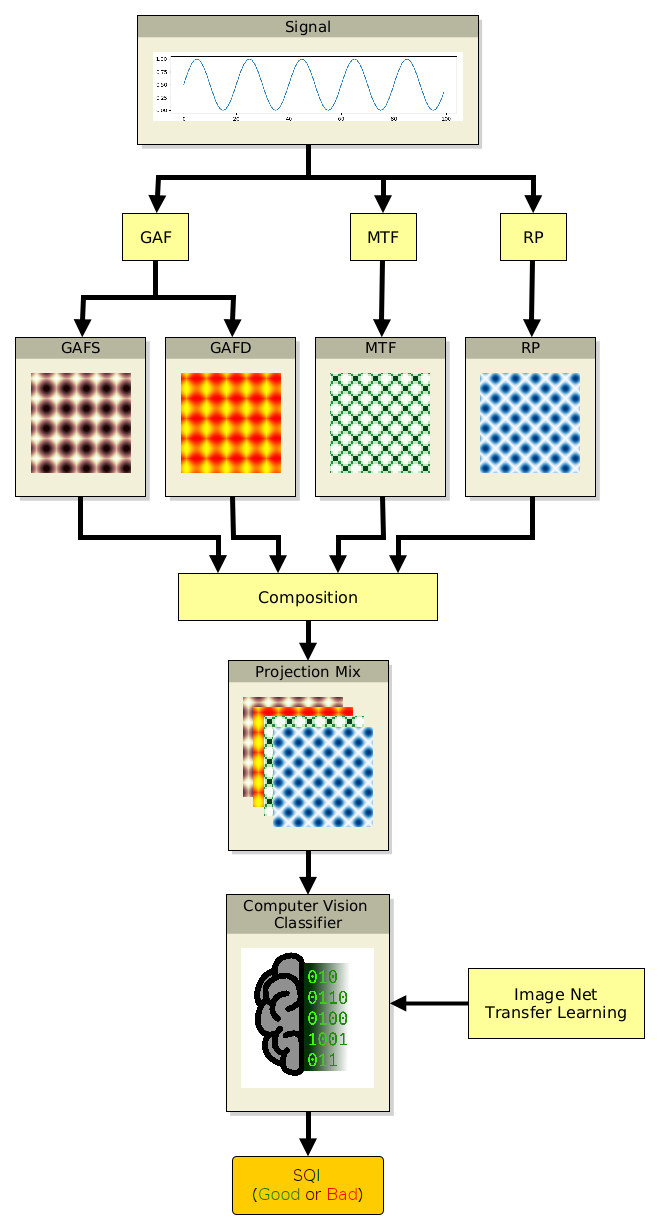
\includegraphics[height=0.95\textheight]{img/method.png}
	\caption{The proposed method. It mainly consisted in feeding the projection composition to the pre-trained \gls{CV} model.}
	\label{fig:method}
\end{figure}




\section{Projection Methods}

This section provides an analysis of the projections methods that this thesis used to convert the one-dimensional \gls{PPG} signal into a 2D representation. For example purposes, we will use the signal in figure \ref{fig:methodology:signal}. Additionally, this section explores the influence of noise in the projections result. 

\begin{figure}[h]
	\centering
	\adjustbox{height=0.3\textheight}{
		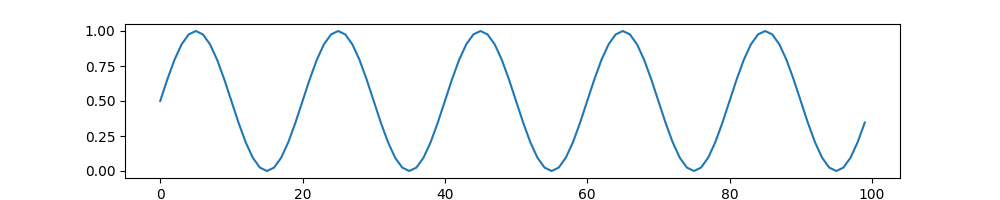
\includegraphics{img/methodology/signal.png}
	}
	\label{fig:methodology:signal}
	\caption{The example signal, with function $f(t)=\sin(\frac{15 \pi t}{500}) + \frac{t}{500}$. }
\end{figure}


\subsection{Recurrence Plot}

The work of Eckmann et al. \cite{rp-1}, of 1987, introduced the \gls{RP} method as a tool for representing visually useful properties and behaviors of a time series. Since then, its application expanded to various domains, ranging areas such as earth sciences, finances, engineering, chemistry and physics \cite{rp-2}. It also is applicable in life sciences, with attemps on identifying the presence of Parkinson's disease \cite{rp-3}, epileptic seizure \cite{rp-4}, fetal hypoxia \cite{rp-5}, and Alzheimer's disease \cite{rp-6}. Particularly, considering this thesis scope, we can employ \gls{RP} in tasks involving cardiological signal processing, such as cardiac arrhythmia classification \cite{rp-7}. Thus, it is likely that this method is useful in the \gls{SQA} of cardiological signals.  

The \gls{RP}, in essence, represents the occurrence of recurrences between the phase space values of time instant pairs. For this end, the first step is to embed the time series $X=\{x_1,x_2,...,x_n\}$, with $ x_i \in \mathbb{R}$ and $n \in \mathbb{N}$ samples, into a phase space, creating a new time series $S=\vec{s_1},\vec{s_2},...,\vec{s_m}$, with $ \vec{s_i} \in \mathbb{R}^d$ and $m \in \mathbb{N}$ elements. We can employ the time delays method to represent each element $\vec{s_i}$ of this new sequence $S$ as follows:

\begin{equation}
    \vec{s_i} = (x_i, x_{i + \tau}, x_{i + 2\cdot \tau} ..., x_{i + (d-1) \cdot \tau})
\end{equation}   

\noindent where $d \in \mathbb{N}$ is the dimension and $\tau \in \mathbb{N}$ is the time delay of the phase space. Notice that the lenght $m$ of the sequence $S$ depends on both $d$ and $\tau$ by the equation $m = n - (d-1) \cdot \tau$. Also notice that this embedding is optional, since the choice of the dimension $d=1$ results in $S=X$, the original time series. The figure \ref{fig:phase_space} depicts the phase space of the example signal of the figure \ref{fig:methodology:signal}.

\begin{figure}[h!]
    \centering
    \adjustbox{width=\textwidth}{
        \begin{tabular}{cc}
            \includegraphics[height=0.2\textheight]{img/methodology/delay_phase_space.pdf} &
            \includegraphics[height=0.2\textheight]{img/methodology/delay_phase_space_recurrences.pdf} 
        \end{tabular}
    }
    \caption{On the left, we have the signal of the figure \ref{fig:methodology:signal} on the time delay phase space, without temporal information. Its parameters are dimension $d=2$ and delay $\tau=\RPDelay$. On the right, we have almost the same figure, but with the recurrences represented by red lines $\vec{s_i} - \vec{s_j}$ that links the pair of near points that have a distance bellow $\varepsilon=\RPThreshold$. That figure omits the recurrences to the point itself.}
    \label{fig:phase_space}
\end{figure}


Then, the second step is to build a $m \times m$ matrix $RP$ of recurrences where each cell $RP_{i,j} \in \{0,1\}$ represents the presence or the ausence of a recurrence in a pair of points $\vec{s_i},\vec{s_j}$ of the phase space $S$. We can represent this concept by measuring the distance $||\vec{s_i} - \vec{s_j}||$ between the points of the pair and verifying if it is smaller than a threshold $\varepsilon \in \mathbb{R}$, as the following equation:

\begin{equation}
    RP_{i,j} = \mathcal{H}(\varepsilon - ||\vec{s_i} - \vec{s_j}||)
\end{equation}

\noindent where $\mathcal{H}: \mathbb{R} \mapsto \{0,1\}$ is the Heaviside function. Alternativelly, we can produce an unthresholded version $RP'_{m \times m}$ by attributing to each cell $RP'_{i,j} \in \mathbb{R}$ the points distance:

\begin{equation}
    RP'_{i,j} = ||\vec{s_i} - \vec{s_j}||
\end{equation}  

\noindent the figure \ref{fig:method:rp} exhibits both $RP$ and $RP'$ of the example signal.

\begin{figure}[h!]
	\centering
	\begin{tabular}{cc}
		\frame{
\includegraphics[width=0.35\textwidth]{img/methodology/RecurrencePlot.png}} &
		\frame{\includegraphics[width=0.35\textwidth]{img/methodology/RecurrencePlotUnthresholded.png}} 
	\end{tabular}
	\caption[The resulting recurrence plots of the signal in Figure \ref{fig:methodology:signal}.]{The resulting recurrence plots of the signal in Figure \ref{fig:methodology:signal}, in coherence with the phase space of the Figure \ref{fig:phase_space}. On the left, we have the thresholded version, while on the right we have the unthresholded version.}
	\label{fig:method:rp}
\end{figure}


\subsection{Gramian Angular Field}

The work of Oates et al. \cite{gaf-mtf-1} introduced the \gls{GAF} method. This method, in summary, encodes the signal into angular relationships between pair of points. The first step to do this is to convert the signal $X=\{x_1,x_2,...,x_n\}$, with $x_i \in \mathbb{R}$, $n \in \mathbb{N}$ samples, and time instants $\{t_1,t_2,...,t_n\}$, into a polar coordinate series $P=\{p_1,p_2,...,p_n\}$ with $p_i \in \mathbb{R}$. One manner to do that is to associate the time $i \in \mathbb{N}$ to the radius $r_i \in \mathbb{R}$ and the value $x_i \in \mathbb{R}$ to the angle by the inverse of the cosine as follows:

\begin{equation}
    p_i = f_{polar}(t_i, x_i) = (r_i, \phi_i),    
    \begin{cases} 
        \phi_i = arccos(x_i), & -1 \leq x_i \leq 1 \wedge 0 \leq \phi_i \leq \pi\\
        r_i = \frac{t_i}{N},     & N \in \mathbb{R}
    \end{cases}
\end{equation}    

\noindent where $N$ is a rescaling factor. Notice that it might be necessary to rescale the signal to fit each $x_i$ in the range $[-1,1]$. The figure \ref{fig:methodology:polar} shows the application of the function $f_{polar}$ over the example signal. The polar coordinate system has one property of interest: the $f_{polar}: \mathbb{N} \times \{x \in \mathbb{R}| -1 \leq x \leq 1\} \mapsto \mathbb{R} \times \{\phi \in \mathbb{R}| 0 \leq \phi \leq \pi \}$ is bijective, since it has the inverse function $f_{polar}^{-1}(r_i, \phi_i)=(r_i \cdot N, cos(\phi_i))=(t_i,x_i)$. This indicates that the application of the function $f_{polar}$ does not result in loss of information.

\begin{figure}[h!]
	\centering
	\adjustbox{width=0.6\textwidth}{
		\includegraphics[trim={4cm 4cm 4cm 4cm}, clip]{img/methodology/polar.png}
	}
	\label{fig:methodology:polar}
	\caption[The example signal in its polar coordinate shape.]{The example signal in its polar coordinate shape, with $N=1$. }
\end{figure}


The second step is to construct the temporal relationship matrix. We can achieve that by two methods that exploit trigonometric properties. One of them is calculating the cosine of the summation of the pairs of angles, constructing the following matrix $GASF_{n \times n}$:

\begin{align}
    GASF_{i,j}     & = cos(\phi_i + \phi_j) \\
            & = cos(\phi_i) \cdot cos(\phi_j) - sin(\phi_i) \cdot sin(\phi_j) \\
            & = x_i \cdot x_j - \sqrt{1 - x_i^2} \cdot \sqrt{1 - x_j^2} \label{eq:gasf:algebraic}
\end{align}

\noindent where \gls{GASF} is the final matrix. Due to the inversibility of the $arccos$ function, it is possible to express that calculation without trigonometric operations, as expressed by the equality \ref{eq:gasf:algebraic}. Thus, we can calculate \gls{GASF} using matrix operations, as follows:  

\begin{equation}
    GASF = X^T \cdot X - \sqrt[\circ 2]{\mathds{1}-X^{\circ 2}}^T \cdot \sqrt[\circ 2]{\mathds{1}-X^{\circ 2}}
\end{equation}

\noindent where $\square^{\circ 2}$ and $\sqrt[\circ 2]{\square}$ represents the element-wise square power and square root of the matrix $\square$, respectivelly, and $\mathds{1}$ is a matrix in which all elements are $1$. The other method is analogous, but uses the sine of the difference of the pairs of angles, constructing the following matrix $GADF_{n \times n}$:

\begin{align}
    GADF_{i,j} & = sin(\phi_i - \phi_j) \\
        & = sin(\phi_i) \cdot cos{\phi_j} - cos(\phi_i) \cdot sin(\phi_j) \\
        & = \sqrt{1 - x_i^2} \cdot x_j - x_i \cdot \sqrt{1 - x_j^2}  \label{eq:gadf:algebraic}
\end{align}

\noindent Also similarly, by the equality \ref{eq:gadf:algebraic}, we can express \gls{GADF} by matrix operations:

\begin{equation}
    GADF = \sqrt[\circ 2]{\mathds{1} - X^{\circ 2}}^T \cdot X - X^T \cdot \sqrt[\circ 2]{\mathds{1} - X^{\circ 2}}
\end{equation}

\noindent the figure \ref{fig:method:gaf} shows the \gls{GASF} and the \gls{GADF} of the example signal.

\begin{figure}
	\centering
	\adjustbox{width=\textwidth}{
		\begin{tabular}{cc}
			\frame{\includegraphics{img/methodology/GramianAngularField(difference).png}} &
			\frame{\includegraphics{img/methodology/GramianAngularField(summation).png}} 
		\end{tabular}
	}
	\caption{The example signal corresponding \gls{GADF} (on the left) and \gls{GASF} (on the right).}
	\label{fig:method:gaf}
\end{figure}


\subsection{Markov Transition Field}

\begin{figure}[h!]
    \centering
    \adjustbox{width=\textwidth}{
	    \begin{tabular}{cc}
		\includegraphics[width=0.5\textwidth, trim={5em 0 5em 0}, clip]{img/methodology/QuantileBins.png} &
		\includegraphics[width=0.5\textwidth, trim={2em 0 3em 0}, clip]{img/methodology/Reconstruction.pdf} \\
		(a) Original signal segmented into quantile bins & (b) Reconstructed example signal
	    \end{tabular}
    }
    \caption{Example of original signal segmented into bands corresponding to eight quantile bins and its reconstruction.}
    \label{fig:method:mtf_signals}
\end{figure}


Oates et al. \cite{gaf-mtf-1} proposed the \gls{MTF} as well, based on a signal to graph mapping of Campanharo et al. \cite{mtf-1}. In fact, that mapping is the first step of this method. We map the signal $X=x_1,x_2,...,x_n$, with $x_i \in \mathbb{R}$, to a graph $G=(N,W)$, with nodes set $N$ and edges weights adjacency matrix $W$. Its nodes $N$ corresponds to $m \in \mathbb{N}$ quantile bins $Q_i \subseteq \{x_i | i \in \{1,2,...,n\}\}$, that is, $|Q_1|=|Q_2|=...=|Q_n|$ and, $\forall q_1 \in Q_1, \forall q_2 \in Q_2, ..., \forall q_n \in Q_n$, we have that $q_1 \leq q_2 \leq ... \leq q_n$. In other words, those quantiles bins separate the signal $X$ into bands $Q_i$ with equal ammount of samples $x_i$. The figure \ref{fig:method:mtf_signals} pictures this concept for the example signal. The other graph component, its edges, are directed and corresponds to the probability of a sample $x_{k+1}$, consecutive to a uniformly randomly chosen sample of a certain quantile $x_k \in Q_i$ (must have a consecutive), belonging to a certain quantile $Q_j$. Those edges are akin to transitions of first-order Markov chains, since the probabilities summation of the transitions that sources from a state is always equal to $100\%$. We can express the adjacency matrix $W_{m \times m}$ as follows:  
\begin{equation}
    W_{i,j} = \frac{
            \sum\limits_{x_k \in Q_i} \begin{cases} 
                0, & x_{k+1} \not\in Q_j \\
                1, & x_{k+1} \in Q_j
            \end{cases}
        }{
            \sum\limits_{Q_l \in Q}\sum\limits_{x_k \in Q_i} \begin{cases} 
                0, & x_{k+1} \not\in Q_l \\
                1, & x_{k+1} \in Q_l
            \end{cases}
        }
\end{equation}

\begin{figure}
	\centering
	\adjustbox{height=0.5\textheight}{\includegraphics{img/methodology/MarkovChain.pdf}}
	\caption{ The graph of the Markov chain representing the transitions of the signal depicted in Figure~\ref{fig:method:mtf_signals}.}
	\label{fig:method:markov_chain}
\end{figure}


\noindent The figure \ref{fig:method:markov_chain} depicts the graph of the example signal. That graph $G$ allows a probabilistic reconstruction $X' = \{ x'_1,x'_2,...,x'_n \}$ of the input signal $X$ by procedurally chosing a sample of the current quantile node and, then, transitioning to the next node according to the transitions probabilities. The algoritm \ref{alg:mtf_reconstruction} explicits that reconstruction and the figure \ref{fig:method:mtf_signals} exemplifies it applied to the example signal. Therefore, the signal conversion to that graph representation is probabilistically reversible, meaning that it preserves statistical information of the signal, even though that means the sucessful recovery is not certain.

\begin{algorithm}
    \begin{algorithmic}
        \Require Graph $G=(N=\{Q_1, Q_2, ..., Q_m\},W)$
        \Ensure Reconstructed Signal $X'=x'_1,x'_2,...,x'_n$
        \State $Q_{current} \gets Q \in_R N$ 
        \For {$k \in 1,2,...,n$}
            \State $x'_k \gets x \in_R Q_{current}$
            \State $Q_{current} \gets Q_{next}$, with probability $W_{current,next}$
        \EndFor
    \end{algorithmic}
    \caption{The probabilistic signal reconstruction algorithm. }
    \label{alg:mtf_reconstruction}
\end{algorithm}

Since that graph does not retain temporal relationships, the second step of the \gls{MTF} method is to build the following matrix $MTF_{n \times n}$: 

\begin{equation}
    MTF_{i,j} = W_{u,v} | x_i \in Q_u, x_j \in Q_v
\end{equation}

\noindent That is, each cell $MTF_{i,j}$ contains the transition probability between the quantiles $Q_u,Q_v$ to which the samples $x_i,x_j$ belong. The figure \ref{fig:method:mtf} pictures the final result of the method applied to the example signal. 

\begin{figure}[h!]
    \centering
    \adjustbox{width=0.4\textwidth}{\frame{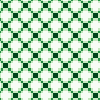
\includegraphics{img/methodology/MarkovTransitionField.png}}}
    \caption[The \acrlong{MTF} of the example signal.]{The \acrlong{MTF} of the example signal, with the number of quantile bins $m=8$.}
    \label{fig:method:mtf}
\end{figure}


\subsection{Projections Comparison}

The main idea of the projection methods is to reflect the signals properties and shape into visual patterns. That concept applies too to the inspection of the signal quality. The figure \ref{fig:method:noises} presents examples of the influence of different type of noises over the projections aspect. On observation is that the presence of low-frequency or high-frequency noises tend to produce, respectively, big or small scale structures. We can see in the effects of that observation in the figure, where the baseline wander figures manifest two to four big structures and the high-frequency noise figures contain small dot-like structures. Another observation is that noises concentrated in a certain region tends to disturb the projection onto a cross-like structure, as we can see in the figure local noise column. We can see that property of ``reflection'' for usual noises, such as Gaussian, and salt and pepper noises. In the figure, the Gaussian noise still preserves the high-level structures and destroys low-level structures, while the salt and pepper noise produces vertical and horizontal lines with void or full colors in places corresponding to, respectively ``salts'' and ``peppers'' of the source signal. Therefore, those projections are likely to be useful in \gls{SQI} tasks for \gls{CV} approaches, since they present the noises visually while maintaining its characteristics.  


\newcommand{\NoisesImageWidth}{0.2\textwidth}

\begin{figure}
	\centering
	\adjustbox{width=\textwidth}{
		\begin{tabular}{cccccc}
			Base signal
			& Gaussian Noise
			& \makecell{Salt and Peper \\Noise}
			& Baseline Wander 
			& \makecell{High-Frequency \\Noise}
			& Local Noise \\
			
			\includegraphics[width=\NoisesImageWidth]{img/methodology/examples/signal(base).png}
			& \includegraphics[width=\NoisesImageWidth]{img/methodology/examples/signal(gaussian).png}
			& \includegraphics[width=\NoisesImageWidth]{img/methodology/examples/signal(salt_and_pepper).png} 
			& \includegraphics[width=\NoisesImageWidth]{img/methodology/examples/signal(baseline_wander).png} 
			& \includegraphics[width=\NoisesImageWidth]{img/methodology/examples/signal(low_frequency_noise).png} 
			& \includegraphics[width=\NoisesImageWidth]{img/methodology/examples/signal(local_noise).png} \\
			
			\frame{\includegraphics[width=\NoisesImageWidth]{img/methodology/examples/GramianAngularDifferenceField(base).png}}
			& \frame{\includegraphics[width=\NoisesImageWidth]{img/methodology/examples/GramianAngularDifferenceField(gaussian).png}} 
			& \frame{\includegraphics[width=\NoisesImageWidth]{img/methodology/examples/GramianAngularDifferenceField(salt_and_pepper).png}} 
			& \frame{\includegraphics[width=\NoisesImageWidth]{img/methodology/examples/GramianAngularDifferenceField(baseline_wander).png}} 
			& \frame{\includegraphics[width=\NoisesImageWidth]{img/methodology/examples/GramianAngularDifferenceField(low_frequency_noise).png}} 
			& \frame{\includegraphics[width=\NoisesImageWidth]{img/methodology/examples/GramianAngularDifferenceField(local_noise).png}} \\
			
			\frame{\includegraphics[width=\NoisesImageWidth]{img/methodology/examples/GramianAngularSummationField(base).png}}
			& \frame{\includegraphics[width=\NoisesImageWidth]{img/methodology/examples/GramianAngularSummationField(gaussian).png}} 
			& \frame{\includegraphics[width=\NoisesImageWidth]{img/methodology/examples/GramianAngularSummationField(salt_and_pepper).png}} 
			& \frame{\includegraphics[width=\NoisesImageWidth]{img/methodology/examples/GramianAngularSummationField(baseline_wander).png}} 
			& \frame{\includegraphics[width=\NoisesImageWidth]{img/methodology/examples/GramianAngularSummationField(low_frequency_noise).png}} 
			& \frame{\includegraphics[width=\NoisesImageWidth]{img/methodology/examples/GramianAngularSummationField(local_noise).png}} \\
			
			\frame{\includegraphics[width=\NoisesImageWidth]{img/methodology/examples/RecurrencePlotUnthresholded(base).png}}
			& \frame{\includegraphics[width=\NoisesImageWidth]{img/methodology/examples/RecurrencePlotUnthresholded(gaussian).png}} 
			& \frame{\includegraphics[width=\NoisesImageWidth]{img/methodology/examples/RecurrencePlotUnthresholded(salt_and_pepper).png}} 
			& \frame{\includegraphics[width=\NoisesImageWidth]{img/methodology/examples/RecurrencePlotUnthresholded(baseline_wander).png}} 
			& \frame{\includegraphics[width=\NoisesImageWidth]{img/methodology/examples/RecurrencePlotUnthresholded(low_frequency_noise).png}} 
			& \frame{\includegraphics[width=\NoisesImageWidth]{img/methodology/examples/RecurrencePlotUnthresholded(local_noise).png}} \\
			
			\frame{\includegraphics[width=\NoisesImageWidth]{img/methodology/examples/MarkovTransitionField(base).png}}
			& \frame{\includegraphics[width=\NoisesImageWidth]{img/methodology/examples/MarkovTransitionField(gaussian).png}} 
			& \frame{\includegraphics[width=\NoisesImageWidth]{img/methodology/examples/MarkovTransitionField(salt_and_pepper).png}} 
			& \frame{\includegraphics[width=\NoisesImageWidth]{img/methodology/examples/MarkovTransitionField(baseline_wander).png}} 
			& \frame{\includegraphics[width=\NoisesImageWidth]{img/methodology/examples/MarkovTransitionField(low_frequency_noise).png}} 
			& \frame{\includegraphics[width=\NoisesImageWidth]{img/methodology/examples/MarkovTransitionField(local_noise).png}} 
		\end{tabular}
	}
	\caption{The signal and its projections over the influence of different type of noises.}
	\label{fig:method:noises}
\end{figure}


\section{Computer Vision Using Projection Mix}

Since each projection has its unique characteristics, they are combined into an ensemble. For this end, all projections are fused toi create an aggregated tensor. This tensor is analogous to a hyperspectral image, i.e., unlike a typical color image, which consists of only three bands (red, green, and blue), the produced tensor provides additional spectral information for each pixel. The aggregation consists in the assignment of each projection to a particular channel of a single input layer. Then, we ``mix'' that aggregation by performing a pointwise convolution operation as illustrated in Figure~\ref{fig:input_layer}. Formally, given $p$ projections $\{M_1, M_2, ..., M_p\}$ with same dimensions $n \times m$, we construct an input tensor $T_{in_{p \times n \times m}}$ defined as follows:
\begin{equation}
    T_{in_{k,i,j}} = M_{k_{i,j}}
\end{equation}
\noindent Then, we ``mix'' that tensor $T_{in}$ into a new tensor $T_{mix_{q \times n \times m}}$ defined bellow:
\begin{equation}
    T_{mix_{k,i,j}} = f_{actv}\left(\sum\limits_{l=1}^{p}T_{in_{l,i,j}} \cdot w_{(k,i,j);l}\right)
\end{equation} 
\noindent where $w_{(k,i,j);l} \in \mathbb{R}$ is the weight applied to the link between the final tensor cell $T_{mix_{k,i,j}}$ and the input tensor cell $T_{in_{l,i,j}}$, while $f_{actv}: \mathbb{R} \mapsto \mathbb{R}$ is an activation function, such as ReLU, logistic sigmoid and Softmax. We can define the same tensor by directly assigning to the input projections:
\begin{equation}
    \label{eq:mix}
    T_{mix_{k,i,j}} = f_{actv}\left(\sum\limits_{l=1}^{p}M_{l_{i,j}} \cdot w_{(k,i,j);l}\right)
\end{equation}
\noindent We can observe that, for each cell with indexes $i,j$, the summatory $\sum\limits_{l=1}^{p}M_{l_{i,j}} \cdot w_{(k,i,j);l}$ ``mixes'' the $p$ projections by adding its values $M_{l_{i,j}}$, while attributing different degrees of contribution for each $l$-th projection depending on the weight $w_{(k,i,j);l}$. Then, we can use the $f_{actv}$ function to mainly achieve binary distinguishability, leading to the final tensor value $T_{mix_{k,i,j}}$. 


\begin{figure}[h!]
	\centering
	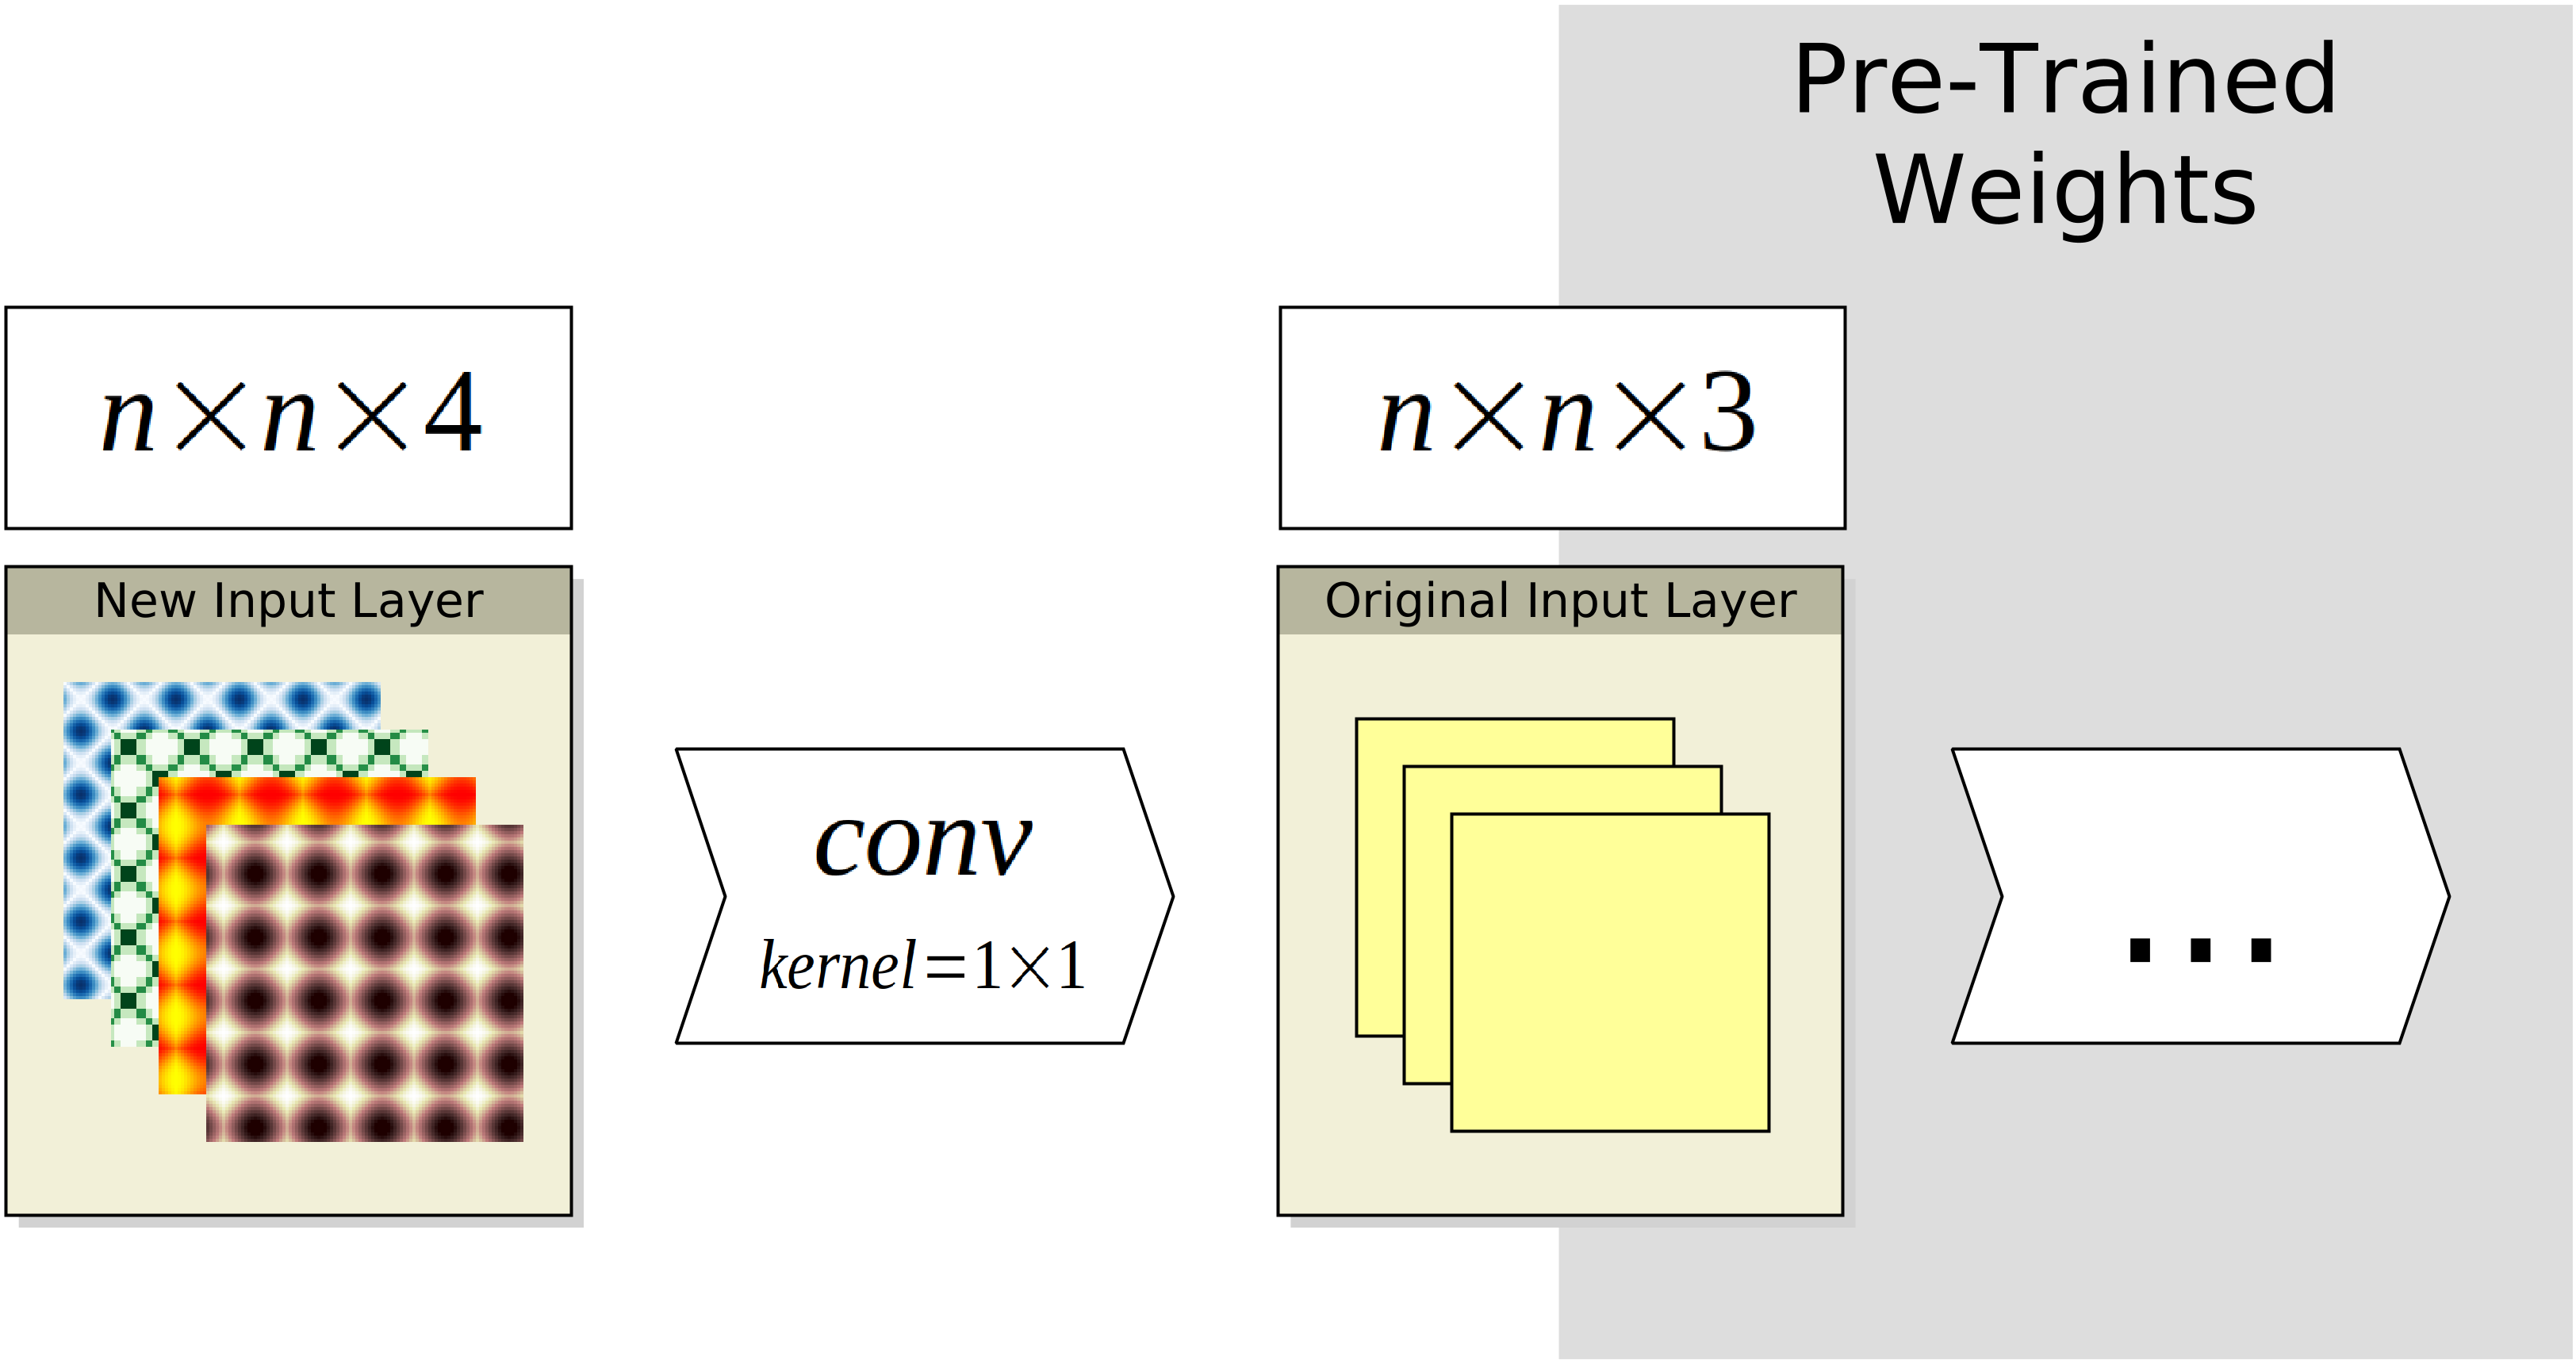
\includegraphics[width=0.8\textwidth]{img/input_layer.png}
	\caption[The three-channeled \acrlong{CV} model feeding process.]{The three-channeled \acrlong{CV} model feeding process. The figure begins in the left, in its input, and progresses to the right. }
	\label{fig:input_layer}
\end{figure}



%\begin{itemize}
%    \item Datasets $\mathcal{D}=\{D_1,D_2,...,D_d\}$
%    \item Signal $X \in \bigcup\limits_{i=1}^d D_i$
%    \item Tensor $\mathcal{T}_{c \times n \times m}$
%    \item Weights set $\mathcal{W}$
%    \item Machine learning model $\mathcal{M}: \mathcal{T}_{c \times n \times m} \times \mathcal{W} \mapsto \{0,1\}$
%    \item $h_{W}(T_{c \times n \times m})=\mathcal{M}(T_{c \times n \times m},W)$
%    \item $\mathcal{P}=\{p_1,p_2,...,p_c\}$
%    \item $p: \bigcup\limits_{i=1}^d D_i \mapsto \mathcal{T}_{c \times n \times m}$
%    \item $h_{W} \circ p: \bigcup\limits_{i=1}^d D_i\mapsto \{0,1\}$
%\end{itemize}

%That projection combination has the property of not only expanding the amount of input options that a machine learning model can use to decide the \gls{SQI}, but also allows, theoretically, a collaboration among the diverse projection methods. Per example, suppose that we want to assess the signal quality on $d$ different datasets, $\mathcal{D}=\{D_1,D_2,...,D_d\}$. To achieve such a goal, we use a machine learning model $\mathcal{M}: \mathcal{T}_{c \times n \times m} \times \mathcal{W} \mapsto \{0,1\}$ which receives an input tensor $T_{c \times n \times m}$ in the set of all tensors with such dimensions $\mathcal{T}_{c \times n \times m}$ and processes it using a weight configuration $W \in \mathcal{W}$, giving an \gls{SQI} in $\{0,1\}$. For simplicity, we define $h_{W}(T_{c \times n \times m})=\mathcal{M}(T_{c \times n \times m},W)$ as the hypothesis function that results from the usage of the model $\mathcal{M}$ with weights $W$. Then, we select a set of projection method function $p: \bigcup\limits_{i=1}^d D_i \mapsto \mathcal{T}_{c \times n \times m}$ in the set $\mathcal{P}=\{p_1,p_2,...,p_c\}$ to convert the signal $X \in \bigcup\limits_{i=1}^d D_i$ to a format compatible with $\mathcal{M}$. The combination of both the model $\mathcal{M}$, with hypothesis function $h_{W}$, and the projection $p$ results in the function composition $h_{W} \circ p: \bigcup\limits_{i=1}^d D_i\mapsto \{0,1\}$ that directly maps the input to the \glspl{SQI}. With that context that this paragraph exposes, one expects that, for each dataset $D \in \mathcal{D}$, a projection method $p_{D} \in \mathcal{P}$ performs equal or better than the others methods. , trained with a function $t_{best}: \mathcal{W} \times \mathcal{D} \mapsto \mathcal{W}$ that retrieves the best set of weights $W_{train} \in \mathcal{W}$

%000000000000000000000000000

%That comes from the implication that the \gls{Mix} method function $p_{mix}(X,W_{mix},f_{act})=T_{mix}(X)$ can produce tensors equivalent to the other projections tensors $T(X)_1$ and $T(X)_2$. Firstly, we use the identity function $f_{id}(x)=x$ as the activation function $f_{actv}$. That and the fact that we use only two projections simplify the equation \ref{eq:mix} to: 

%\begin{align}
%    T(X)_{mix_{k,i,j}} = & f_{actv}\left(\sum\limits_{l=1}^{2}M(X)_{l_{i,j}} \cdot w_{(k,i,j);l}\right) \\
%    T(X)_{mix_{k,i,j}} = & f_{id}\left(\sum\limits_{l=1}^{2}M(X)_{l_{i,j}} \cdot w_{(k,i,j);l}\right) \\
%    T(X)_{mix_{k,i,j}} = & \sum\limits_{l=1}^{2}M(X)_{l_{i,j}} \cdot w_{(k,i,j);l} \\
%    T(X)_{mix_{k,i,j}} = & M(X)_{1_{i,j}} \cdot w_{(k,i,j);1} + M(X)_{2_{i,j}} \cdot w_{(k,i,j);2}
%\end{align}

%We can observe that, when a set of weights $W_{{mix}_1}$ such that $w_{(k,i,j);1}=1$ and $w_{(k,i,j);2}=0$, we have that $T(X)_{mix_{k,i,j}} = M(X)_{1_{i,j}}$, that is, $T(X)_{mix}=T(X)_1$. Similarly, with weights $W_{{mix}_2}$ such that $w_{(k,i,j);1}=0$ and $w_{(k,i,j);2}=1$, it can also assume the values of $T(X)_2$. Therefore, $T(X)_{mix}$ can assume the value of both projection methods with the same projection method. Consequently, when we assume that the training over the weights $W_{mix}$ in a initial state $W_{{mix}_0}$, represented by a function $f(D,W_{{mix}_0})=W_{mix}$, produces the  assume both $W_{{mix}_1}$ and $W_{{mix}_2}$ 

